% OWNER: empirical
% STATUS: draft
% SOURCES: notes/HIPOTEZY_REWIZJA.md; plan analiz rozdz. 6; eksport danych (do wstawienia)
\chapter{Wyniki badań}
\label{ch08:top}
\ChapterStatus{draft}{empirical}

Raportuję tu ewaluację terenową artefaktu IDA (warstwa~C dowodu; por.\ rozdz.~\ref{ch06:sec:warstwy}, \ref{ch07:top}) według pytań \RQ{1}--\RQ{6}.
Kolejność odpowiada planowi analiz z~\cref{tab:ch06:rq}: najpierw próba i jakość danych, potem wyniki dla każdego pytania, na końcu zestawienie w tabeli.
Liczby pochodzą z odczytu Cloud SQL (\texttt{awa\_db}) z~1~października 2026 (wyłącznie \texttt{SELECT}; identyfikatory uczestników nie wchodzą do tekstu).
Ostatnia aktualizacja rekordu \texttt{participants} tego dnia przypada na 11:39 czasu warszawskiego.
Próba jest mała, więc podaję częstości, mediany i rho Spearmana jako opis pilotażu. Modele konfirmacyjne i twierdzenia psychometryczne odkładam do większego~$N$ (por.\ rozdz.~\ref{ch06:sec:statystyka}).

\section{Charakterystyka próby i jakość danych}
\label{ch08:sec:proba}

\paragraph{Kryteria włączenia do analiz.}
Za punkt wyjścia biorę rekordy z ważną zgodą badawczą (\texttt{consent\_timestamp} niepusty; por.\ rozdz.~\ref{ch06:sec:etyka}). Przy każdym pytaniu liczę tylko osoby z kompletem pól, których to pytanie wymaga (na przykład \texttt{blind\_selection\_made} dla~\RQ{3}).
Ścieżki \texttt{full} i \texttt{fast} podaję osobno wszędzie tam, gdzie ich porównanie ma sens (\RQ{1},~\RQ{6}).

\paragraph{Wielkość próby i wykruszanie się uczestników.}
W \texttt{participants} jest 240 wierszy ze znacznikiem zgody: ścieżka \texttt{fast} 109, \texttt{full} 85, bez \texttt{path\_type} 46.
Ścieżki nie są tym samym lejkiem. Na \texttt{full} profil rdzeniowy ma 68 z 85 osób, wynik liczbowy Big Five (\texttt{big5\_openness} niepusty) 39, pokój 49, ślepy wybór 16, ankietę satysfakcji 25.
Znacznik \texttt{big5\_completed\_at} jest ustawiony u 174 osób (84 full, 89 fast), ale wynik domen jest zapisany tylko u 42 (39 full, 3 fast). Do porównań osobowości używam wyniku liczbowego, nie samej flagi ukończenia.
Na \texttt{fast} generację ma 61 ze 109 osób, profil rdzeniowy 4, ślepy wybór 1, satysfakcję 2. Czterdzieści sześć rekordów bez ścieżki ma zapisaną zgodę i niemal nic poza nią (jeden z nich zawiera zapis selekcji kart).

\paragraph{Lejek ukończenia.}
Rycina~\ref{fig:ch08:funnel} pokazuje kamienie milowe ścieżki \texttt{full} ($N=85$), czyli tej, na której opiera się macierz. Spadek nie następuje w jednym miejscu: afektywna selekcja kart (74) i preferencje jawne (71) są częstsze niż uzupełniony pokój (49), a flaga Big Five (84) jest prawie powszechna przy 39 zapisanych wynikach.

\begin{figure}[htbp]
  \centering
  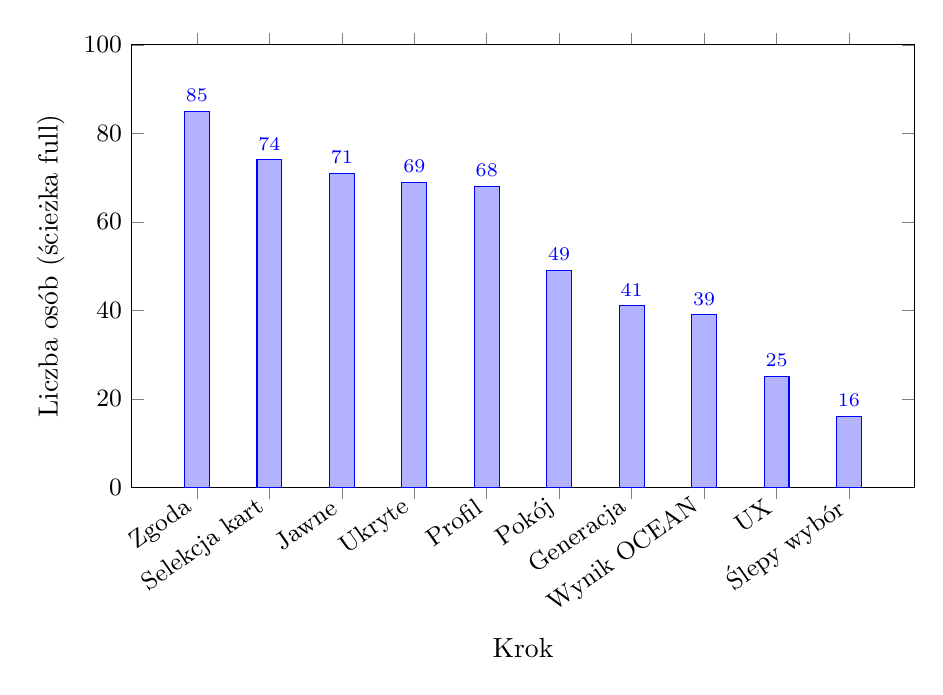
\begin{tikzpicture}
    \begin{axis}[
      ybar,
      bar width=9pt,
      width=0.95\linewidth,
      height=7.2cm,
      ylabel={Liczba osób (ścieżka full)},
      xlabel={Krok},
      symbolic x coords={Zgoda,Swipy,Jawne,Ukryte,Profil,Pokoj,Generacja,OCEAN,UX,Wybor},
      xticklabels={Zgoda,{Selekcja kart},Jawne,Ukryte,Profil,Pokój,Generacja,{Wynik OCEAN},UX,{Ślepy wybór}},
      xtick=data,
      x tick label style={rotate=35,anchor=east,font=\small},
      ymin=0, ymax=100,
      nodes near coords,
      every node near coord/.append style={font=\scriptsize,/pgf/number format/fixed},
      tick label style={font=\small},
    ]
    \addplot coordinates {
      (Zgoda,85) (Swipy,74) (Jawne,71) (Ukryte,69) (Profil,68)
      (Pokoj,49) (Generacja,41) (OCEAN,39) (UX,25) (Wybor,16)
    };
    \end{axis}
  \end{tikzpicture}
  \caption{Kamienie milowe ścieżki \texttt{full} ($N=85$). Oś kategorii: krok zapisu. Oś wartości: liczba osób. Stan bazy 1 października 2026. „Wynik OCEAN” oznacza niepusty \texttt{big5\_openness}, nie samą flagę \texttt{big5\_completed\_at}.}
  \label{fig:ch08:funnel}
\end{figure}

\paragraph{Jakość danych behawioralnych i profilu.}
W \texttt{participant\_swipes} jest 2190 zdarzeń u 74 osób i każde ma \texttt{reaction\_time\_ms}. Mediana czasu reakcji wynosi 1609~ms (kwartyle 1074 i 2513). Mediana liczby ocenionych kart na osobę wynosi 30 (oba kwartyle też 30), czyli zadanie ma stałą długość. W lewo poszło 1303 gestów (mediana 1623~ms), w prawo 887 (mediana 1599~ms).
\texttt{preference\_comparison\_json} jest niepusty u 180 osób. \texttt{style\_match} jest prawdziwy tylko u 10, wszystkie na ścieżce full; fałszywy u 170, w tym u wszystkich 108 rekordów fast z tym JSON-em. Ścieżka fast prawie nie zbiera gestów selekcji kart i preferencji jawnych (po 5 osób), więc fałsz u 108 z nich może wynikać z braku jednego z kanałów, a nie z porównania. Nie traktuję \texttt{style\_match} w tej próbie jako miary rozbieżności.

\paragraph{Ścieżka w zapisie i generacje obrazów.}
Pole \texttt{path\_type} opisuje ostatnią zapisaną ścieżkę w wierszu \texttt{participants}, a nie całą historię sesji. Część osób zaczyna od Fast i przechodzi do Full, dlatego na ścieżce \texttt{fast} w tabeli~\ref{tab:ch08:completeness} widać m.in.\ 89 flag ukończenia Big Five przy zaledwie 4 profilach rdzeniowych --- to pozostałość po dłuższym przebiegu, a nie pełny lejek Fast. W \texttt{participant\_generations} jest 1174 zleceń: 411 zakończonych sukcesem, 485 błędem i 278 w stanie \texttt{pending} (stan bazy 1~października 2026; zestawienie w \cref{ch08:sec:snapshot-2026-10-01}). Wysoki udział błędów i zleceń oczekujących oznacza, że wybór w macierzy mógł dotyczyć podzbioru renderów, które uczestnik faktycznie zobaczył.

\section{RQ1 --- ciągłość doświadczenia dialogowego i kompletność profilu}
\label{ch08:sec:rq1}

\textbf{Pytanie:} czy zintegrowany flow badawczy umożliwia zebranie wielowymiarowego profilu bez katastrofalnego dropoutu? (rozdz.~\ref{ch01:sec:cel}, \ref{ch06:sec:rq}).

\paragraph{Operacjonalizacja.}
Wskaźniki: \texttt{core\_profile\_complete}, \texttt{current\_step}, czas między \texttt{created\_at} a \texttt{updated\_at}, kompletność wymiarów (implicit, explicit, big5, room, macierz), eventy \texttt{page\_view}.

\paragraph{Hipoteza robocza (pilotaż).}
Uczestnicy ścieżki Full z \texttt{core\_profile\_complete} dostarczają komplet danych w kluczowych wymiarach --- bez twierdzenia o walidacji konstruktu skal zgamifikowanych (to nie jest cel~\RQ{1}; por.\ rewizja H1 w notatkach metodologicznych).

\paragraph{Wynik.}
Na ścieżce full odpadanie nie ucina flow na starcie: 68 z 85 osób ma profil rdzeniowy, 74 ukończyło selekcję kart, 71 preferencje jawne i 69 ukryte. Liczba osób spada głównie przy pokoju (49), wyniku liczbowym Big Five (39, przy 84 flagach ukończenia testu) oraz ankiecie UX (25); flaga ślepego wyboru jest u 16 (19\% startu full). Ścieżka fast zbiera zgodę (109) i generację (61), ale prawie nie zbiera profilu rdzeniowego (4) ani macierzy (1), więc nie jest porównywalnym lejkiem badawczym.

\begin{table}[htbp]
  \centering
  \small
  \caption{Kompletność zapisu według ścieżki, 1 października 2026.}
  \label{tab:ch08:completeness}
  \begin{tabular}{lrrrr}
    \toprule
    Krok & full (85) & fast (109) & brak ścieżki (46) & razem \\
    \midrule
    Zgoda & 85 & 109 & 46 & 240 \\
    Profil rdzeniowy & 68 & 4 & 0 & 72 \\
    Selekcja kart & 74 & 5 & 1 & 80 \\
    Preferencje jawne & 71 & 5 & 0 & 76 \\
    Preferencje ukryte & 69 & 25 & 0 & 94 \\
    Wynik Big Five & 39 & 3 & 0 & 42 \\
    Ślepy wybór & 16 & 1 & 0 & 17 \\
    Satysfakcja & 25 & 2 & 0 & 27 \\
    \bottomrule
  \end{tabular}
\end{table}

\paragraph{Status interpretacyjny.}
Odpowiedź na~\RQ{1} w tym zrzucie: flow full da się przejść do profilu i preferencji bez katastrofalnego odpadnięcia na starcie. Komplet wieloźródłowy (osobowość z wynikiem, ślepa macierz, UX) jest już wyraźnie mniejszy. Fast nie dostarcza tej samej kompletności.

\section{RQ2 --- rozbieżność implicit vs explicit a zachowanie w macierzy}
\label{ch08:sec:rq2}

\textbf{Pytanie:} czy i w jakim stopniu preferencje ukryte i jawne się rozchodzą, oraz czy ta rozbieżność wiąże się z zachowaniem w macierzy generacji?

Ramę teoretyczną stanowią procesy dualne i pomiar asocjacji ukrytych \footcite{kahneman2011thinking,greenwald1998iat} oraz model wieloźródłowy z rozdz.~\ref{ch03:top}; operacjonalizacja rozbieżności --- rozdz.~\ref{ch06:sec:instrumenty}, \ref{ch07:sec:macierz}.

\paragraph{Operacjonalizacja.}
{\sloppy Zmienne: \texttt{preference\_comparison\_json}, \texttt{style\_match}, \allowbreak\texttt{color\_tokens\_match\_score}, \texttt{selected\_source}, \texttt{selection\_time\_ms}, \texttt{conflict\_analysis}, wpisy \allowbreak\texttt{participant\_matrix\_entries}.\par}

\paragraph{Hipotezy robocze.}
\begin{itemize}
  \item \Hyp{2a}: wyższy mismatch $\rightarrow$ dłuższy \texttt{selection\_time\_ms} lub częstszy wybór \texttt{mixed} / \texttt{mixed\_functional};
  \item \Hyp{2b}: przy \texttt{style\_match = false} rzadszy wybór źródła \texttt{explicit}.
\end{itemize}

\paragraph{Wynik (pilotaż: opis rozkładów; nie regresja jako główny wniosek).}
Na skalach ciągłych implicit i explicit idą w tę samą stronę, a nie przeciw sobie. Rho Spearmana, osoby z oboma pomiarami ($n=72$): ciepło 0,39, jasność 0,46, złożoność 0,43.
\texttt{style\_match = true} ma tylko 10 osób, wszystkie full. Wśród wyborów macierzy na full przy \texttt{style\_match = false} źródło \texttt{explicit} wybrano 2 razy na 17 zaznaczeń; przy \texttt{true} 1 raz na 6. Przy takich liczebnościach \Hyp{2b} nie daje się ocenić. W \texttt{generation\_feedback} jest 59 wierszy z polem \texttt{selected\_source}; 58 z nich ma \texttt{conflict\_analysis}. Nie testuję tu związku rozbieżności z czasem wyboru ani z wyborem \texttt{mixed}.

\paragraph{Status interpretacyjny.}
W tym zrzucie skale implicit i explicit są zgodne co do kierunku, a etykiety stylu w \texttt{conflict\_analysis} często się rozjeżdżają. Związku rozbieżności z wyborem mixed nie da się tu potwierdzić: komórek jest za mało, a \texttt{style\_match} jest prawie wszędzie fałszywy.

\section{RQ3 --- wybór źródła w ślepej macierzy (rdzeń empiryczny)}
\label{ch08:sec:rq3}
\label{ch08:sec:macierz}

\textbf{Pytanie:} które źródło w ślepej macierzy sześciu wariantów użytkownicy wybierają i czy wybór zależy od profilu?

To oś empiryczna rozprawy (por.\ rozdz.~\ref{ch01:sec:teza}, \ref{ch07:sec:slepy-wybor}): zmienna zależna to \texttt{generation\_feedback.selected\_source}, nie ogólna satysfakcja.

\paragraph{Operacjonalizacja.}
{\sloppy \texttt{selected\_source}, \texttt{generated\_sources}, \allowbreak\texttt{has\_complete\_bigfive}, \texttt{inspirations\_count}, \allowbreak\texttt{blind\_selection\_made}.\par}

\paragraph{Hipotezy robocze (confirmatory po większym~$N$).}
\begin{itemize}
  \item \Hyp{3a}: \texttt{mixed} lub \texttt{mixed\_functional} częściej niż źródła „czyste”;
  \item \Hyp{3b}: kompletne Big Five $\leftrightarrow$ częstszy wybór \texttt{personality} lub \texttt{mixed};
  \item \Hyp{3c}: $\geq 1$ inspiracja $\leftrightarrow$ częstszy wybór \texttt{inspiration\_reference}.
\end{itemize}

\paragraph{Wynik.}
{\sloppy Wybór zapisują trzy liczniki i nie sumują się one do tej samej liczby osób. \allowbreak\texttt{generation\_feedback.selected\_source}: 59 wierszy. \allowbreak\texttt{participant\_matrix\_entries.is\_selected}: 29 osób (po jednym zaznaczeniu). Flaga \allowbreak\texttt{blind\_selection\_made} jest ustawiona u 17 osób (16 na ścieżce full). Rycina~\ref{fig:ch08:selected-source} pokazuje wiersze feedbacku, bo tak jest nazwana zmienna zależna w planie. Tabela obok podaje zaznaczenia macierzy, czyli osoby. Dodatkowo interfejs w części sesji pokazywał tylko odblokowane karty wizji (bramka konta; rozdz.~\ref{ch07:sec:slepy-wybor}), więc wybór nie zawsze oznacza porównanie pełnej siatki sześciu obrazów.\par}

\begin{figure}[htbp]
  \centering
  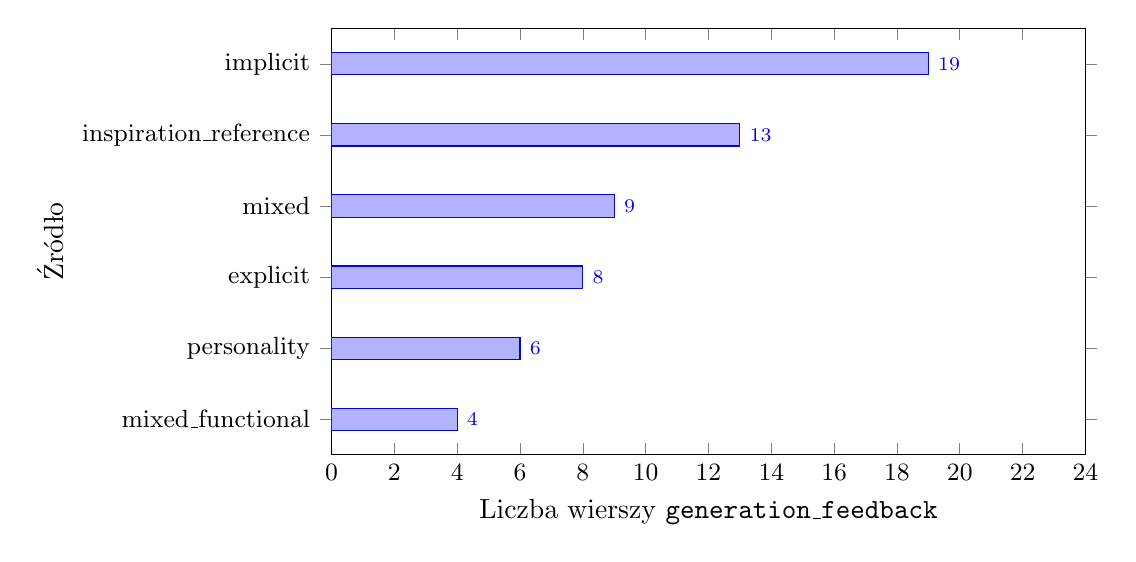
\begin{tikzpicture}
    \begin{axis}[
      xbar,
      bar width=8pt,
      width=0.92\linewidth,
      height=7cm,
      xlabel={Liczba wierszy \texttt{generation\_feedback}},
      ylabel={Źródło},
      symbolic y coords={mf,personality,explicit,mixed,inspiration,implicit},
      ytick=data,
      yticklabels={mixed\_functional,personality,explicit,mixed,inspiration\_reference,implicit},
      xmin=0, xmax=24,
      nodes near coords,
      every node near coord/.append style={font=\scriptsize},
      tick label style={font=\small},
    ]
    \addplot coordinates {
      (4,mf) (6,personality) (8,explicit)
      (9,mixed) (13,inspiration) (19,implicit)
    };
    \end{axis}
  \end{tikzpicture}
  \caption{Wybory źródła w \texttt{generation\_feedback} (59 wierszy). Oś kategorii: \texttt{selected\_source}. Oś wartości: liczba wierszy, nie liczba osób. Stan bazy 1 października 2026.}
  \label{fig:ch08:selected-source}
\end{figure}

\begin{table}[htbp]
  \centering
  \small
  \caption{Zaznaczenie w macierzy (\texttt{is\_selected}), 29 osób, oraz wiersze feedbacku.}
  \label{tab:ch08:sources}
  \begin{tabular}{lrrrr}
    \toprule
    Źródło & osoby w macierzy & \% z 29 & wiersze feedbacku & \% z 59 \\
    \midrule
    implicit & 11 & 38 & 19 & 32 \\
    mixed & 6 & 21 & 9 & 15 \\
    inspiration\_reference & 5 & 17 & 13 & 22 \\
    explicit & 3 & 10 & 8 & 14 \\
    personality & 2 & 7 & 6 & 10 \\
    mixed\_functional & 2 & 7 & 4 & 7 \\
    \bottomrule
  \end{tabular}
\end{table}

\noindent
\Hyp{3a} w tym zrzucie nie wychodzi: mixed i mixed\_functional razem to 13 z 59 wierszy feedbacku i 8 z 29 osób w macierzy, a samo implicit jest częstsze (19 wierszy, 11 osób).
Z 29 osób z zaznaczeniem wynik Big Five ma 21; źródło personality wybrały 2 i obie mają wynik. To za mało na \Hyp{3b}.
Wszystkie 5 osób, które w macierzy wybrały inspiration\_reference, miało co najmniej jedną inspirację; inspirację miało też 6 z 11 osób wybierających implicit. \Hyp{3c} jest zgodne z kierunkiem w tej komórce, ale $n=5$.

\paragraph{Status interpretacyjny.}
W pilotażu najczęściej wskazywane źródło to implicit, nie wariant mieszany. Trzy liczniki (feedback, macierz, flaga ślepego wyboru) trzeba trzymać osobno, dopóki nie zostanie ustalone, który jest wyborem końcowym.

\section{RQ4 --- osobowość a wybór wariantu i parametry estetyczne}
\label{ch08:sec:rq4}
\label{ch08:sec:personality}

\textbf{Pytanie:} czy cechy i ich podwymiary Big Five wiążą się z parametrami estetycznymi profilu oraz z preferencją źródła \texttt{personality}?

Rama: taksonomia OCEAN i IPIP-NEO-120 w IDA (rozdz.~\ref{ch05:top}; \cite{john2008bigfive}); status analiz --- \emph{eksploracyjny} przy małym~$N$.

\paragraph{Hipotezy robocze (H4a--c).}
Asocjacje \texttt{big5\_openness} z~\texttt{implicit\_complexity} / stylem; \texttt{big5\_conscientiousness} z~\texttt{explicit\_*}; wybór \texttt{personality} przy ekstremalnych wartościach domen --- bez progu $r\!>\!0{,}4$ jako claimu potwierdzającego.

\paragraph{Wynik.}
Wynik domen jest u 42 osób (39 full). Pary poniżej to rho Spearmana; przy $n=41$--42 są to asocjacje eksploracyjne, nie potwierdzenie progu $r>0{,}4$.

\begin{table}[htbp]
  \centering
  \small
  \caption{Rho Spearmana: domeny Big Five a skale estetyczne. Eksploracja, 1 października 2026.}
  \label{tab:ch08:big5}
  \begin{tabular}{llrr}
    \toprule
    Para & kierunek z hipotezy & $n$ & rho \\
    \midrule
    otwartość $\times$ złożoność implicit & H4a, plus & 41 & 0,20 \\
    otwartość $\times$ ciepło implicit & poza H4a & 41 & 0,35 \\
    ugodowość $\times$ ciepło implicit & poza planem & 41 & 0,41 \\
    sumienność $\times$ złożoność explicit & H4b & 41 & $-0{,}29$ \\
    sumienność $\times$ ciepło explicit & H4b & 42 & 0,02 \\
    neurotyczność $\times$ złożoność implicit & poza planem & 41 & 0,29 \\
    \bottomrule
  \end{tabular}
\end{table}

\noindent
H4a (otwartość i złożoność implicit) jest słabe. Silniejszy związek otwartości w tym zbiorze dotyczy ciepła implicit, a nie złożoności. Sumienność nie idzie z ciepłem jawnym; ze złożonością jawną znak jest ujemny i niewielki.
Źródło personality w macierzy wybrały 2 osoby, obie z wynikiem Big Five. Rho otwartości z wyborem personality (1/0 wśród 21 osób z wynikiem i zaznaczeniem) wynosi 0,43, ale przy dwóch wyborach jeden wysoki wynik otwartości przesuwa współczynnik. \Hyp{4c} zostaje nieocenione.
Podwymiarów (aspektów cech) nie raportuję: \texttt{big5\_facets} przy niepustym wyniku jest obiektem, ale nie ma tu stabilnej serii do heatmapy.

\paragraph{Status interpretacyjny.}
Eksploracja pilotażowa nie podtrzymuje H4a w postaci „otwartość $\rightarrow$ złożoność”. Widać umiarkowane rho ciepła implicit z otwartością i ugodowością. Wybór personality jest za rzadki, żeby z niego wnioskować.

\section{RQ5 --- luka PRS (\texorpdfstring{current$\rightarrow$target}{current-target}) a wybór mixed\_functional}
\label{ch08:sec:rq5}

\textbf{Pytanie:} czy odległość PRS \texttt{current}$\rightarrow$\texttt{target} wiąże się z preferencją wariantu \texttt{mixed\_functional}?

To \textbf{nie} jest klasyczny pre/post regeneracyjności po AI (stary H2 odrzucony przy braku \texttt{prs\_post\_*}; por.\ rozdz.~\ref{ch02:top}, \ref{ch06:sec:ograniczenia}).
Konstrukt luki nastrojowej łączy się z ART / mapowaniem mood grid \footcite{kaplan1995restorative}.

\paragraph{Operacjonalizacja.}
Odległość euklidesowa z~\texttt{prs\_current\_*} i~\texttt{prs\_target\_*}; DV: \texttt{selected\_source} (w szczególności \texttt{mixed\_functional}).

\paragraph{Hipoteza robocza \Hyp{5a}.}
Większa luka PRS $\rightarrow$ częstszy wybór \texttt{mixed\_functional}.

\paragraph{Wynik.}
Odległość euklidesowa current$\rightarrow$target na obu osiach jest policzalna u 47 osób. Średnia luka wynosi 0,68 (współrzędne mood gridu, nie punkty skali PRS-11).
Wśród osób z luką i zaznaczeniem w macierzy średnia luka wynosi: implicit 0,39 ($n=10$), mixed 0,36 ($n=5$), explicit 0,52 ($n=2$), inspiration\_reference 0,82 ($n=5$), personality 0,23 ($n=2$), mixed\_functional 0,04 ($n=1$). Dwadzieścia dwie osoby z luką nie mają zaznaczenia; ich średnia luka jest wyższa (0,94).
Rho luki z wyborem mixed\_functional (1/0, $n=25$ osób z luką i jakimkolwiek zaznaczeniem) wynosi $-0{,}28$. Jedyna osoba, która wybrała mixed\_functional i ma obie osie PRS, ma lukę bliską zera. To jest kierunek przeciwny do \Hyp{5a} i komórka $n=1$.

\paragraph{Status interpretacyjny.}
\Hyp{5a} w tym zrzucie nie ma oparcia. Brak pomiaru po ekspozycji na obraz pozostaje ograniczeniem schematu, nie wnioskiem o regeneracyjności.

\section{RQ6 --- doświadczenie użytkownika (agency, clarity, satisfaction)}
\label{ch08:sec:rq6}

\textbf{Pytanie:} czy uczestnicy postrzegają proces jako zrozumiały i dający sprawczość przy jednoczesnym zbieraniu danych badawczych?

\paragraph{Operacjonalizacja.}
{\sloppy Skale \texttt{agency\_*}, \texttt{clarity\_*}, \allowbreak\texttt{satisfaction\_*}, \texttt{sus\_*}; \texttt{path\_type} (Full vs Fast).\par}

\paragraph{Hipotezy robocze.}
\Hyp{6a}: dodatnia korelacja agency/clarity z satisfaction; \Hyp{6b}: Full vs Fast --- tylko przy wystarczającej liczbie ścieżek Fast.

\paragraph{Wynik.}
Ankieta pochodzi prawie wyłącznie ze ścieżki full. Średnie na niepustych wartościach w ścieżce full: SUS 66,48 ($n=27$), zrozumiałość procesu (\texttt{clarity\_*}) 5,05 ($n=26$), sprawczość 5,13 ($n=25$), satysfakcja 5,34 ($n=25$). Na fast są dwie osoby (SUS 68,75, satysfakcja 5,38), więc \Hyp{6b} nie ma próby.
Rho Spearmana ze satysfakcją: sprawczość 0,71 ($n=27$), zrozumiałość 0,68 ($n=26$), SUS 0,77 ($n=27$). Sprawczość ze zrozumiałością: 0,57 ($n=26$). \Hyp{6a} ma w tym pilotażu zgodny kierunek i największe współczynniki w całym rozdziale, przy $n$ około 27.

\paragraph{Status interpretacyjny.}
Osoby, które doszły do ankiety, wiążą sprawczość i zrozumiałość procesu z satysfakcją. To nie jest próba wszystkich 240 rekordów i nie rozdziela satysfakcji według źródła obrazu.

\section{Wskaźniki behawioralne (ograniczenie względem dawnego H5)}
\label{ch08:sec:behavioral}

Dawna hipoteza o wyższości dwell/hesitation nad samym gestem swipe \textbf{nie jest operacjonalizowana} w obecnym schemacie --- w bazie persystowane jest przede wszystkim \texttt{reaction\_time\_ms} (por.\ rozdz.~\ref{ch03:top}, \ref{ch06:sec:trafnosc}).

\paragraph{Zakres dopuszczalnej analizy.}
Czas reakcji jest kompletny: 2190 z 2190 gestów selekcji kart. Mediana 1609~ms, kwartyle 1074 i 2513. Gest w lewo i w prawo ma niemal ten sam czas (1623~ms i 1599~ms), więc samo \texttt{reaction\_time\_ms} nie rozdziela polubienia od odrzucenia. Nie ma w tym zrzucie osobnego czasu wahania ani dwell. Nie łączę czasu pojedynczego gestu wyboru karty z \texttt{selection\_time\_ms} macierzy: to inne zadanie i inne $n$.

\section{Analizy dodatkowe}
\label{ch08:sec:dodatkowe}

\paragraph{Konflikty preferencji.}
\texttt{conflict\_analysis} jest w 58 z 59 wierszy feedbacku. W 47 z 58 etykieta stylu implicit różni się od etykiety explicit. To pokrywa się z opisem przy~\RQ{2}; nie dorzucam tu osobnej typologii konfliktów.

\paragraph{Ścieżka Fast vs Full.}
Full: 85 osób, 16 ślepych wyborów, 25 ankiet satysfakcji. Fast: 109 osób, 1 ślepy wybór, 2 ankiety, za to 61 osób z generacją. Porównanie UX i macierzy między ścieżkami nie ma liczebności po stronie fast (rozdz.~\ref{ch06:sec:procedura}, \ref{ch07:sec:sciezki}).

% Snapshot zagregowany z Cloud SQL (awa_db), 1 października 2026, 13:16 Europe/Warsaw.
% Ostatnia aktualizacja rekordu participants: 2026-10-01 09:39:10 UTC.
% Zapytania: data/snapshot-2026-10-01.sql
% Wstawienie: % Snapshot zagregowany z Cloud SQL (awa_db), 1 października 2026, 13:16 Europe/Warsaw.
% Ostatnia aktualizacja rekordu participants: 2026-10-01 09:39:10 UTC.
% Zapytania: data/snapshot-2026-10-01.sql
% Wstawienie: % Snapshot zagregowany z Cloud SQL (awa_db), 1 października 2026, 13:16 Europe/Warsaw.
% Ostatnia aktualizacja rekordu participants: 2026-10-01 09:39:10 UTC.
% Zapytania: data/snapshot-2026-10-01.sql
% Wstawienie: \input{chapters/08-dane-2026-10-01} wewnątrz rozdziału Wyniki.
\section{Stan zbioru na 1 października 2026}
\label{ch08:sec:snapshot-2026-10-01}

\paragraph{Źródło.}
Liczby poniżej pochodzą z agregacji tabel badawczych w Cloud SQL (baza \texttt{awa\_db}), wykonanej 1~października 2026 o~13:16 czasu warszawskiego. Eksport nie zawiera identyfikatorów uczestników. Pierwszy rekord w \texttt{participants} powstał 13~marca 2026; ostatnia aktualizacja rekordu przypada na 1~października 2026, 11:39 czasu warszawskiego. To opis stanu operacyjnego zbioru, nie zamknięta próba analityczna z~rozdziału metodologii.

\begin{table}[ht]
  \centering
  \caption{Wolumen tabel badawczych, stan na 1 października 2026}
  \label{tab:ch08:volume-2026-10-01}
  \begin{tabular}{lr}
    \toprule
    Tabela & $N$ \\
    \midrule
    \texttt{participants} & 240 \\
    \texttt{research\_consents} & 249 \\
    \texttt{participant\_swipes} & 2190 \\
    \texttt{participant\_generations} & 1174 \\
    \texttt{participant\_research\_events} & 4354 \\
    \texttt{participant\_matrix\_entries} & 143 \\
    \bottomrule
  \end{tabular}
\end{table}

\paragraph{Ścieżka i kompletność.}
W~\texttt{participants} jest 240 wierszy: ścieżka \texttt{fast} --- 109, ścieżka \texttt{full} --- 85, brak \texttt{path\_type} --- 46. Znacznik czasu zgody jest przy wszystkich 240 wierszach. Eksport sesji (\texttt{session\_export\_json}) ma 185 osób, w~tym 77 na ścieżce pełnej i~108 na szybkiej. Ukończony Big Five (\texttt{big5\_completed\_at}) ma 174 osoby, w~tym 84 na ścieżce pełnej i~89 na szybkiej. Profil rdzeniowy (\texttt{core\_profile\_complete}) ma 72 osoby, z~czego 68 na ścieżce pełnej. Flaga ślepego wyboru (\texttt{blind\_selection\_made}) jest ustawiona u~17 osób, w~tym u~16 na ścieżce pełnej.

\begin{table}[ht]
  \centering
  \caption{Kamienie milowe w \texttt{participants} według ścieżki (1 października 2026)}
  \label{tab:ch08:path-2026-10-01}
  \begin{tabular}{lrrrrr}
    \toprule
    Ścieżka & $N$ & profil rdzeniowy & Big Five & eksport sesji & ślepy wybór \\
    \midrule
    \texttt{fast} & 109 & 4 & 89 & 108 & 1 \\
    \texttt{full} & 85 & 68 & 84 & 77 & 16 \\
    brak & 46 & 0 & 1 & 0 & 0 \\
    \midrule
    Razem & 240 & 72 & 174 & 185 & 17 \\
    \bottomrule
  \end{tabular}
\end{table}

\paragraph{Napływ.}
Nowe rekordy \texttt{participants} według miesiąca utworzenia (czas warszawski): marzec 6, kwiecień 7, maj 1, czerwiec 40, lipiec 3, sierpień 35, wrzesień 148. Wrzesień jest jedynym miesiącem o~wyraźnej skali rekrutacji. W~samym oknie 21~września--1~października aktualizowano kolejno 1, 12, 6, 41, 25, 10, 2, 13, 19, 1 i~1 rekordów; szczyt aktualizacji przypada na 24~września (41).

\paragraph{Ślepa macierz.}
Tabela \texttt{participant\_matrix\_entries} ma 143 wiersze. Flaga \texttt{is\_selected} jest ustawiona w~29 wierszach, każdy u~innej osoby. Rozkład zaznaczeń: \texttt{implicit} 11, \texttt{mixed} 6, \texttt{inspiration\_reference} 5, \texttt{explicit} 3, \allowbreak\texttt{mixed\_functional} 2, \texttt{personality} 2. To nie jest to samo co \allowbreak\texttt{blind\_selection\_made} w~\texttt{participants} ($n=17$). Do wniosków o~RQ3 potrzebne jest uzgodnienie obu znaczników, zanim którykolwiek z~nich zostanie uznany za wybór końcowy.

\paragraph{Afektywna selekcja kart i zadania generacji.}
W~tabeli \texttt{participant\_swipes} zapisano 2190 zdarzeń: 1303 odrzucenia (gest w~lewo) i~887 akceptacji (gest w~prawo); łącznie 80 osób wykonało co najmniej jeden gest wyboru w module afektywnej selekcji kart. W~\texttt{participant\_generations} jest 1174 zleceń: 411 zakończonych sukcesem, 485 błędem, 278 w~stanie \texttt{pending}. Udział błędów wynosi 485/1174. Sto dwa rekordy uczestników mają \texttt{generations\_count}~$>0$.

\paragraph{Skale po flow.}
Średnie liczone tylko na niepustych wartościach: SUS 66,64 ($n=29$), jasność 5,00 ($n=28$), sprawczość 5,10 ($n=27$), satysfakcja 5,34 ($n=27$). Przy tak małym $n$ są to opisy rozkładu, nie test różnic między ścieżkami.

\paragraph{Czego ten zrzut nie rozstrzyga.}
Zbiór 240 wierszy miesza sesje testowe, ścieżkę szybką, ścieżkę pełną i~rekordy bez ścieżki. Rdzeń empiryczny ślepego wyboru pozostaje mały ($n=17$ albo $n=29$, zależnie od znacznika). Wysoki udział generacji w~stanie błędu lub \texttt{pending} ogranicza interpretację obrazów jako bodźca, który uczestnik faktycznie zobaczył.
 wewnątrz rozdziału Wyniki.
\section{Stan zbioru na 1 października 2026}
\label{ch08:sec:snapshot-2026-10-01}

\paragraph{Źródło.}
Liczby poniżej pochodzą z agregacji tabel badawczych w Cloud SQL (baza \texttt{awa\_db}), wykonanej 1~października 2026 o~13:16 czasu warszawskiego. Eksport nie zawiera identyfikatorów uczestników. Pierwszy rekord w \texttt{participants} powstał 13~marca 2026; ostatnia aktualizacja rekordu przypada na 1~października 2026, 11:39 czasu warszawskiego. To opis stanu operacyjnego zbioru, nie zamknięta próba analityczna z~rozdziału metodologii.

\begin{table}[ht]
  \centering
  \caption{Wolumen tabel badawczych, stan na 1 października 2026}
  \label{tab:ch08:volume-2026-10-01}
  \begin{tabular}{lr}
    \toprule
    Tabela & $N$ \\
    \midrule
    \texttt{participants} & 240 \\
    \texttt{research\_consents} & 249 \\
    \texttt{participant\_swipes} & 2190 \\
    \texttt{participant\_generations} & 1174 \\
    \texttt{participant\_research\_events} & 4354 \\
    \texttt{participant\_matrix\_entries} & 143 \\
    \bottomrule
  \end{tabular}
\end{table}

\paragraph{Ścieżka i kompletność.}
W~\texttt{participants} jest 240 wierszy: ścieżka \texttt{fast} --- 109, ścieżka \texttt{full} --- 85, brak \texttt{path\_type} --- 46. Znacznik czasu zgody jest przy wszystkich 240 wierszach. Eksport sesji (\texttt{session\_export\_json}) ma 185 osób, w~tym 77 na ścieżce pełnej i~108 na szybkiej. Ukończony Big Five (\texttt{big5\_completed\_at}) ma 174 osoby, w~tym 84 na ścieżce pełnej i~89 na szybkiej. Profil rdzeniowy (\texttt{core\_profile\_complete}) ma 72 osoby, z~czego 68 na ścieżce pełnej. Flaga ślepego wyboru (\texttt{blind\_selection\_made}) jest ustawiona u~17 osób, w~tym u~16 na ścieżce pełnej.

\begin{table}[ht]
  \centering
  \caption{Kamienie milowe w \texttt{participants} według ścieżki (1 października 2026)}
  \label{tab:ch08:path-2026-10-01}
  \begin{tabular}{lrrrrr}
    \toprule
    Ścieżka & $N$ & profil rdzeniowy & Big Five & eksport sesji & ślepy wybór \\
    \midrule
    \texttt{fast} & 109 & 4 & 89 & 108 & 1 \\
    \texttt{full} & 85 & 68 & 84 & 77 & 16 \\
    brak & 46 & 0 & 1 & 0 & 0 \\
    \midrule
    Razem & 240 & 72 & 174 & 185 & 17 \\
    \bottomrule
  \end{tabular}
\end{table}

\paragraph{Napływ.}
Nowe rekordy \texttt{participants} według miesiąca utworzenia (czas warszawski): marzec 6, kwiecień 7, maj 1, czerwiec 40, lipiec 3, sierpień 35, wrzesień 148. Wrzesień jest jedynym miesiącem o~wyraźnej skali rekrutacji. W~samym oknie 21~września--1~października aktualizowano kolejno 1, 12, 6, 41, 25, 10, 2, 13, 19, 1 i~1 rekordów; szczyt aktualizacji przypada na 24~września (41).

\paragraph{Ślepa macierz.}
Tabela \texttt{participant\_matrix\_entries} ma 143 wiersze. Flaga \texttt{is\_selected} jest ustawiona w~29 wierszach, każdy u~innej osoby. Rozkład zaznaczeń: \texttt{implicit} 11, \texttt{mixed} 6, \texttt{inspiration\_reference} 5, \texttt{explicit} 3, \allowbreak\texttt{mixed\_functional} 2, \texttt{personality} 2. To nie jest to samo co \allowbreak\texttt{blind\_selection\_made} w~\texttt{participants} ($n=17$). Do wniosków o~RQ3 potrzebne jest uzgodnienie obu znaczników, zanim którykolwiek z~nich zostanie uznany za wybór końcowy.

\paragraph{Afektywna selekcja kart i zadania generacji.}
W~tabeli \texttt{participant\_swipes} zapisano 2190 zdarzeń: 1303 odrzucenia (gest w~lewo) i~887 akceptacji (gest w~prawo); łącznie 80 osób wykonało co najmniej jeden gest wyboru w module afektywnej selekcji kart. W~\texttt{participant\_generations} jest 1174 zleceń: 411 zakończonych sukcesem, 485 błędem, 278 w~stanie \texttt{pending}. Udział błędów wynosi 485/1174. Sto dwa rekordy uczestników mają \texttt{generations\_count}~$>0$.

\paragraph{Skale po flow.}
Średnie liczone tylko na niepustych wartościach: SUS 66,64 ($n=29$), jasność 5,00 ($n=28$), sprawczość 5,10 ($n=27$), satysfakcja 5,34 ($n=27$). Przy tak małym $n$ są to opisy rozkładu, nie test różnic między ścieżkami.

\paragraph{Czego ten zrzut nie rozstrzyga.}
Zbiór 240 wierszy miesza sesje testowe, ścieżkę szybką, ścieżkę pełną i~rekordy bez ścieżki. Rdzeń empiryczny ślepego wyboru pozostaje mały ($n=17$ albo $n=29$, zależnie od znacznika). Wysoki udział generacji w~stanie błędu lub \texttt{pending} ogranicza interpretację obrazów jako bodźca, który uczestnik faktycznie zobaczył.
 wewnątrz rozdziału Wyniki.
\section{Stan zbioru na 1 października 2026}
\label{ch08:sec:snapshot-2026-10-01}

\paragraph{Źródło.}
Liczby poniżej pochodzą z agregacji tabel badawczych w Cloud SQL (baza \texttt{awa\_db}), wykonanej 1~października 2026 o~13:16 czasu warszawskiego. Eksport nie zawiera identyfikatorów uczestników. Pierwszy rekord w \texttt{participants} powstał 13~marca 2026; ostatnia aktualizacja rekordu przypada na 1~października 2026, 11:39 czasu warszawskiego. To opis stanu operacyjnego zbioru, nie zamknięta próba analityczna z~rozdziału metodologii.

\begin{table}[ht]
  \centering
  \caption{Wolumen tabel badawczych, stan na 1 października 2026}
  \label{tab:ch08:volume-2026-10-01}
  \begin{tabular}{lr}
    \toprule
    Tabela & $N$ \\
    \midrule
    \texttt{participants} & 240 \\
    \texttt{research\_consents} & 249 \\
    \texttt{participant\_swipes} & 2190 \\
    \texttt{participant\_generations} & 1174 \\
    \texttt{participant\_research\_events} & 4354 \\
    \texttt{participant\_matrix\_entries} & 143 \\
    \bottomrule
  \end{tabular}
\end{table}

\paragraph{Ścieżka i kompletność.}
W~\texttt{participants} jest 240 wierszy: ścieżka \texttt{fast} --- 109, ścieżka \texttt{full} --- 85, brak \texttt{path\_type} --- 46. Znacznik czasu zgody jest przy wszystkich 240 wierszach. Eksport sesji (\texttt{session\_export\_json}) ma 185 osób, w~tym 77 na ścieżce pełnej i~108 na szybkiej. Ukończony Big Five (\texttt{big5\_completed\_at}) ma 174 osoby, w~tym 84 na ścieżce pełnej i~89 na szybkiej. Profil rdzeniowy (\texttt{core\_profile\_complete}) ma 72 osoby, z~czego 68 na ścieżce pełnej. Flaga ślepego wyboru (\texttt{blind\_selection\_made}) jest ustawiona u~17 osób, w~tym u~16 na ścieżce pełnej.

\begin{table}[ht]
  \centering
  \caption{Kamienie milowe w \texttt{participants} według ścieżki (1 października 2026)}
  \label{tab:ch08:path-2026-10-01}
  \begin{tabular}{lrrrrr}
    \toprule
    Ścieżka & $N$ & profil rdzeniowy & Big Five & eksport sesji & ślepy wybór \\
    \midrule
    \texttt{fast} & 109 & 4 & 89 & 108 & 1 \\
    \texttt{full} & 85 & 68 & 84 & 77 & 16 \\
    brak & 46 & 0 & 1 & 0 & 0 \\
    \midrule
    Razem & 240 & 72 & 174 & 185 & 17 \\
    \bottomrule
  \end{tabular}
\end{table}

\paragraph{Napływ.}
Nowe rekordy \texttt{participants} według miesiąca utworzenia (czas warszawski): marzec 6, kwiecień 7, maj 1, czerwiec 40, lipiec 3, sierpień 35, wrzesień 148. Wrzesień jest jedynym miesiącem o~wyraźnej skali rekrutacji. W~samym oknie 21~września--1~października aktualizowano kolejno 1, 12, 6, 41, 25, 10, 2, 13, 19, 1 i~1 rekordów; szczyt aktualizacji przypada na 24~września (41).

\paragraph{Ślepa macierz.}
Tabela \texttt{participant\_matrix\_entries} ma 143 wiersze. Flaga \texttt{is\_selected} jest ustawiona w~29 wierszach, każdy u~innej osoby. Rozkład zaznaczeń: \texttt{implicit} 11, \texttt{mixed} 6, \texttt{inspiration\_reference} 5, \texttt{explicit} 3, \allowbreak\texttt{mixed\_functional} 2, \texttt{personality} 2. To nie jest to samo co \allowbreak\texttt{blind\_selection\_made} w~\texttt{participants} ($n=17$). Do wniosków o~RQ3 potrzebne jest uzgodnienie obu znaczników, zanim którykolwiek z~nich zostanie uznany za wybór końcowy.

\paragraph{Afektywna selekcja kart i zadania generacji.}
W~tabeli \texttt{participant\_swipes} zapisano 2190 zdarzeń: 1303 odrzucenia (gest w~lewo) i~887 akceptacji (gest w~prawo); łącznie 80 osób wykonało co najmniej jeden gest wyboru w module afektywnej selekcji kart. W~\texttt{participant\_generations} jest 1174 zleceń: 411 zakończonych sukcesem, 485 błędem, 278 w~stanie \texttt{pending}. Udział błędów wynosi 485/1174. Sto dwa rekordy uczestników mają \texttt{generations\_count}~$>0$.

\paragraph{Skale po flow.}
Średnie liczone tylko na niepustych wartościach: SUS 66,64 ($n=29$), jasność 5,00 ($n=28$), sprawczość 5,10 ($n=27$), satysfakcja 5,34 ($n=27$). Przy tak małym $n$ są to opisy rozkładu, nie test różnic między ścieżkami.

\paragraph{Czego ten zrzut nie rozstrzyga.}
Zbiór 240 wierszy miesza sesje testowe, ścieżkę szybką, ścieżkę pełną i~rekordy bez ścieżki. Rdzeń empiryczny ślepego wyboru pozostaje mały ($n=17$ albo $n=29$, zależnie od znacznika). Wysoki udział generacji w~stanie błędu lub \texttt{pending} ogranicza interpretację obrazów jako bodźca, który uczestnik faktycznie zobaczył.


\section{Podsumowanie wyników}
\label{ch08:sec:podsumowanie}

Tabela~\ref{tab:ch08:rq-summary} zbiera odpowiedzi na pytania badawcze według odczytu z 1 października 2026.
Siła jest opisowa. Żaden wiersz nie jest testem konfirmacyjnym.

\begin{table}[htbp]
  \centering
  \footnotesize
  \setlength{\tabcolsep}{3.5pt}
  \caption{Synteza wyników \RQ{1}--\RQ{6} według odczytu z 1 października 2026 roku.}
  \label{tab:ch08:rq-summary}
  \begin{tabular}{@{}>{\raggedright\arraybackslash}p{0.08\textwidth}>{\raggedright\arraybackslash}p{0.23\textwidth}>{\raggedright\arraybackslash}p{0.27\textwidth}>{\raggedright\arraybackslash}p{0.17\textwidth}>{\raggedright\arraybackslash}p{0.19\textwidth}@{}}
    \toprule
    RQ & Zagadnienie badawcze & Wynik w pilotażu & Status / siła & Główne ograniczenie \\
    \midrule
    \RQ{1} & Wykonalność przebiegu i kompletność &
    Ścieżka pełna dociera do profilu (68/85); ślepy wybór 16/85 &
    Opis lejka ukończenia &
    Ścieżka szybka nieporównywalna; flaga Big Five $\neq$ wynik \\
    \addlinespace
    \RQ{2} & Rozbieżność ukryte vs jawne a macierz &
    Skale ciągłe zgodne ($\rho = 0{,}39$--$0{,}46$, $n=72$); etykiety stylu różne w 47/58 &
    Opis; \Hyp{2a}--\Hyp{2b} nierozstrzygnięte &
    Zmienna \texttt{style\_match} niemal zawsze fałszywa \\
    \addlinespace
    \RQ{3} & Wybór źródła w ślepej macierzy &
    Najczęściej wariant ukryty \texttt{implicit} (11/29 osób; 19/59 opinii) &
    Brak potwierdzenia \Hyp{3a} w pilotażu &
    Trzy osobne liczniki wyboru; błędy generacji \\
    \addlinespace
    \RQ{4} & Wielka Piątka a estetyka i wybór &
    Otwartość $\times$ złożoność $\rho = 0{,}20$; ciepło $\rho = 0{,}35$; wybór \texttt{personality} $n=2$ &
    Analiza eksploracyjna &
    Mała liczebność komórek wyboru \\
    \addlinespace
    \RQ{5} & Luka nastroju PRS a wariant funkcjonalny &
    $\rho = -0{,}28$ ($n=25$); wybór \texttt{mixed\_functional} z pełną luką $n=1$ &
    Brak oparcia dla \Hyp{5a} &
    Brak pomiaru PRS po ekspozycji na obraz \\
    \addlinespace
    \RQ{6} & Sprawczość, zrozumiałość, satysfakcja &
    Dodatnie korelacje z satysfakcją ($\rho = 0{,}71$ i $0{,}68$, $n \approx 27$) &
    Kierunek zgodny z \Hyp{6a} &
    Satysfakcja mierzona dla sesji; w ścieżce szybkiej $n=2$ \\
    \bottomrule
  \end{tabular}
\end{table}

\paragraph{Czego rozdział świadomie nie raportuje.}
Walidacji zgamifikowanego PRS względem papierowego PRS-11; testów mediacji wielopoziomowych; „poprawy regeneracyjności o~$X$ punktów” po ekspozycji na AI --- zgodnie z ograniczeniami schematu i rewizją hipotez (rozdz.~\ref{ch06:sec:statystyka}).
